\documentclass[a4paper,11pt]{report}

\usepackage{fullpage}

\usepackage{amsmath}
\usepackage{bussproofs}
\usepackage{mathpartir}
\usepackage{prooftrees}
\usepackage{placeins}
\usepackage{color}

% Minted
\usepackage[cache=false]{minted}

\newmintinline{c}{
  fontsize=\small,
  breaklines=true
}

\newminted{c}{
  frame=single,
  framesep=2mm,
  fontsize=\scriptsize,
  mathescape
}

\newminted[clinecode]{c}{
  frame=single,
  framesep=2mm,
  fontsize=\scriptsize,
  mathescape,
  linenos
}

\newcommand*{\BBox}[1]{\draw (#1 + 0.5,0.5) -- (#1 + 1.5,0.5) -- (#1 + 1.5,-0.2)
  -- (#1 + 0.5,-0.2) -- cycle;}
\newcommand*{\SBox}[1]{}

\newcommand*{\equal}{=}

% for finite state automata
\usepackage{tikz}
\usetikzlibrary{automata,positioning}

\author{Sylvain Julmy}
\date{\today}

\setlength{\parindent}{0pt}

\begin{document}

\begin{center}
  \Large{
    System-oriented Programming\\
    Spring 2018
  }
  
  \noindent\makebox[\linewidth]{\rule{\linewidth}{0.4pt}}
  S06
  \noindent\makebox[\linewidth]{\rule{\linewidth}{0.4pt}}

  \begin{flushleft}
    Professor : Philippe Cudré-Mauroux

    Assistant : Michael Luggen
  \end{flushleft}
  
  \noindent\makebox[\linewidth]{\rule{\linewidth}{0.4pt}}

  Submitted by Sylvain Julmy
  
  \noindent\makebox[\linewidth]{\rule{\textwidth}{1pt}}
\end{center}

\section*{Exercise 1}

\subsection*{a)}

\begin{figure}[h]
  \centering
  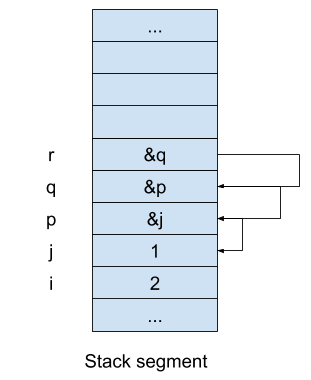
\includegraphics[width=0.3\textwidth]{figures/SOP_s06_ex1_a}
  \caption{\label{fig:ex1-a}}
\end{figure}

\FloatBarrier

\subsection*{b)}

\begin{figure}[h]
  \centering
  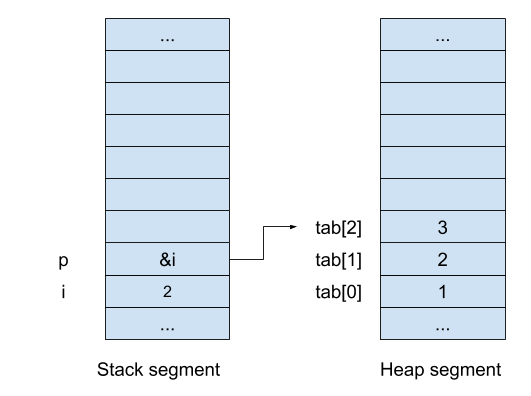
\includegraphics[width=0.5\textwidth]{figures/SOP_s06_ex1_b}
  \caption{\label{fig:ex1-b}}
\end{figure}

\FloatBarrier

\subsection*{c)}

\begin{figure}[h]
  \centering
  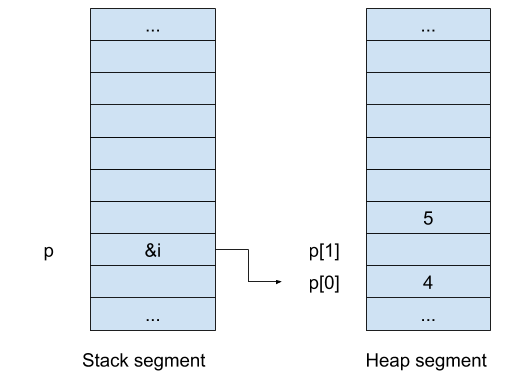
\includegraphics[width=0.5\textwidth]{figures/SOP_s06_ex1_c}
  \caption{\label{fig:ex1-c}}
\end{figure}

\FloatBarrier

\section*{Exercise 2}

\begin{itemize}
\item[a)] $a$ is a local array of local array of int.
\item[b)] $b$ is a local array of pointer on int.
\item[c)] $c$ is a function which take no arguments and return an int. We have
  to specify $void$ for the arguments to garanteed that the function should not
  take any argument.
\item[d)] $d$ is a function which take a pointer of a function which has no
  argument and return an int. The function $d$ return an int as well.
\item[e)] $f$ is a function which return a function that return an int with no
  arguments. The function $f$ take $0$ argument.
\end{itemize}

\section*{Exercise 3}

\begin{itemize}
\item[a)] $stackt$ is a synonym for pointer on void.
\item[b)] $fctInt\_t$ is a synonym for a function which take an int and return
  an int.
\item[c)] $fct\_gen$ is a synonym for a function which take a pointer on void
  and return a pointer on void.
\item[d)] $signal$ is a synonym for a function which take $2$ arguments : an int
  and a function that return nothing and take an int. $signal$ return a function
  that return nothing and take an int.
\end{itemize}

\section*{Exercise 4}

$mult$ return $(2+4) * 8 = 48$. $compute$ return $(2+4) * 8 = 48$

\begin{figure}[h]
  \centering
  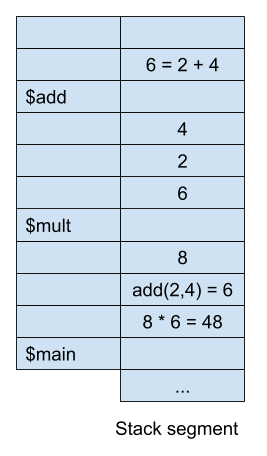
\includegraphics[width=0.3\textwidth]{figures/SOP_s06_ex4_a}
  \caption{\label{fig:ex4-a} Stack segment of $mult$.}
\end{figure}

\begin{figure}[h]
  \centering
  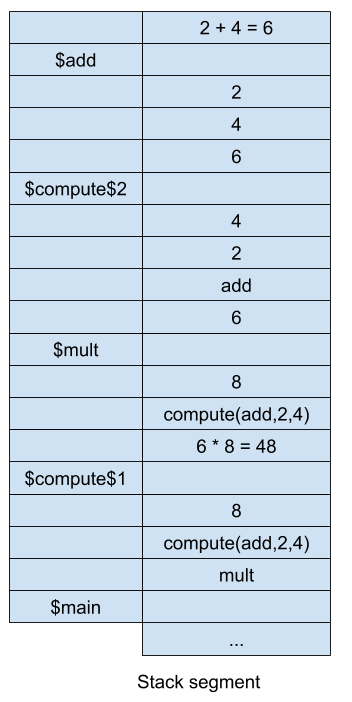
\includegraphics[width=0.3\textwidth]{figures/SOP_s06_ex4_b}
  \caption{\label{fig:ex4-b} Stack segment of $compute$.}
\end{figure}

\FloatBarrier

\section*{Exercise 5}

I think I didn't find the correct code for this exercice...

\begin{figure}[ht]
  \centering
  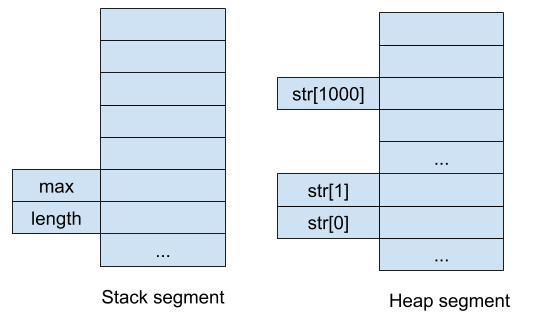
\includegraphics[width=0.6\textwidth]{figures/SOP_s06_ex5}
  \caption{\label{fig:ex5} Stack and heap segment.}
\end{figure}

\end{document}
